\chapter{支持向量机}

本章将介绍支持向量机(SVM)学习算法。SVM 是最好的(许多人甚至认为是最好的)“开箱即用”的监督学习算法之一。为了讲述 SVM 的故事,首先需要讨论间隔 (margin) 以及用大间隔分隔数据的思想。接下来,将讨论最优间隔分类器,这将引出对拉格朗日对偶性的讨论。还将看到核,它允许在非常高维(例如无限维)特征空间中高效地应用 SVM,最后会以 SMO 算法作为结束,该算法提供了 SVM 的高效实现。

\section{间隔:直觉}

我们将从讨论间隔开始讲述 SVM 的故事。本节将给出关于间隔以及预测的“置信度”的直觉;这些思想将在第 \ref{sec:6.3} 节中正式化。

考虑逻辑回归,其中概率 $p(y=1|x; \theta)$ 由 $h_\theta(x) = g(\theta^T x)$ 建模。当且仅当 $h_\theta(x) \ge 0.5$ 时,或者等价地,当且仅当 $\theta^T x \ge 0$ 时,预测输入 $x$ 的标签为“1”。考虑一个正训练样本 ($y=1$)。$\theta^T x$ 越大,$h_\theta(x) = p(y=1|x; \theta)$ 也越大,因此预测标签为 1 的“置信度”也越高。因此,可以非正式地认为,如果 $\theta^T x \gg 0$,则预测非常确信标签为 1。类似地,如果 $\theta^T x \ll 0$,则认为逻辑回归非常确信预测标签为 0。给定一个训练集,再次非正式地看来,如果能找到 $\theta$ 使得当 $y^{(i)}=1$ 时 $\theta^T x^{(i)} \gg 0$,并且当 $y^{(i)}=0$ 时 $\theta^T x^{(i)} \ll 0$,这将反映出一个非常确信(且正确)的分类集,其适用于所有训练样本。这似乎是一个很好的目标,很快将使用函数间隔的概念来形式化这个想法。

为了获得另一种直觉,考虑下面的图,其中 x 表示正训练样本,o 表示负训练样本,还显示了决策边界(这是由方程 $\theta^T x = 0$ 给出的直线,也称为\textbf{分隔超平面 (separating hyperplane)}),并且还标记了三个点 A、B 和 C。

\begin{figure}[H]
    \centering
    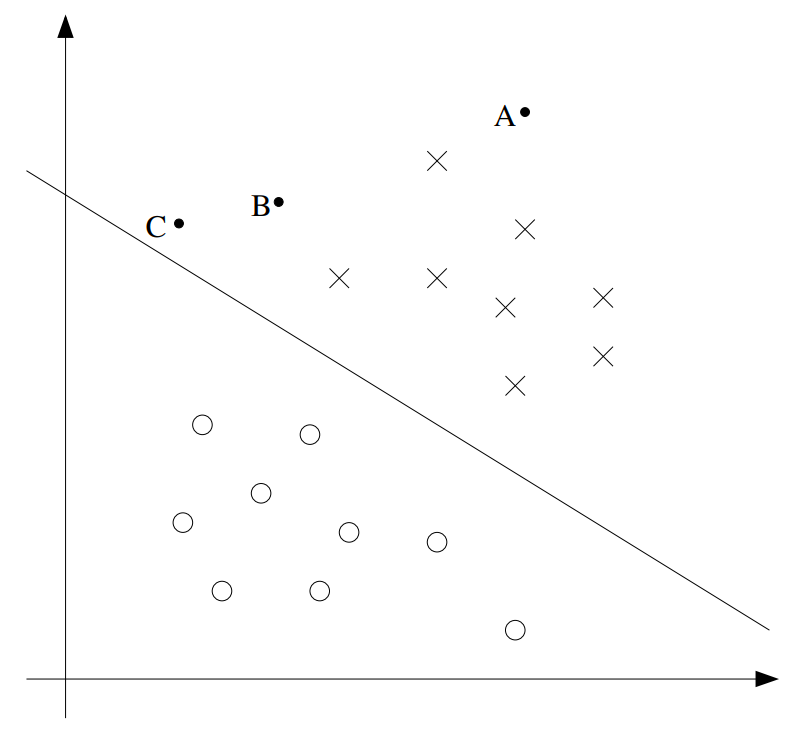
\includegraphics[width=0.5\linewidth]{figs/svm_hyperplane.png}
\end{figure}

注意到点 A 离决策边界非常远。如果要求预测 A 点的 $y$ 值,似乎应该非常确信那里 $y=1$。相反,点 C 离决策边界非常近,尽管它在决策边界预测 $y=1$ 的一侧,但决策边界的微小变化似乎很容易导致预测结果为 $y=0$。因此,在 A 点的预测比在 C 点更确信。点 B 介于这两种情况之间,更广泛地说,可以看出,如果一个点离分隔超平面很远,那么预测可能会更确信。同样,非正式地认为,如果给定一个训练集,能够找到一个决策边界,使得在训练样本上做出所有正确且确信(即远离决策边界)的预测,那将是很好的。稍后将使用几何间隔的概念来形式化这个想法。

\section{符号 (选读)}

为了更容易讨论 SVM,首先需要引入一种新的符号来讨论分类。将考虑一个二元分类问题的线性分类器,其标签为 $y$,特征为 $x$。从现在开始,使用 $y \in \{-1, 1\}$(而不是 $\{0, 1\}$)来表示类别标签。此外,不再使用向量 $\theta$ 来参数化线性分类器,而是使用参数 $w, b$,并将分类器写为
\[
    h_{w,b}(x) = g(w^T x + b).
\]
这里,$g(z) = 1$ 如果 $z \ge 0$,否则 $g(z) = -1$。这种“$w, b$”符号允许将截距项 $b$ 与其他参数分开处理(还放弃了之前让 $x_0 = 1$ 成为输入特征向量中的额外坐标的约定)。因此,$b$ 扮演着之前 $\theta_0$ 的角色,而 $w$ 扮演着 $[\theta_1 \dots \theta_d]^T$ 的角色。

还注意到,根据上面 $g$ 的定义,分类器将直接预测 1 或 -1(参见感知器算法),而无需先经过估计 $p(y=1)$ 的中间步骤(这是逻辑回归所做的)。

\section{函数间隔与几何间隔 (选读)}\label{sec:6.3}

现在将函数间隔和几何间隔的概念形式化。给定一个训练样本 $(x^{(i)}, y^{(i)})$,定义 $(w,b)$ 相对于训练样本的\textbf{函数间隔 (functional margin)}为
\[
    \hat{\gamma}^{(i)} = y^{(i)}(w^T x^{(i)} + b).
\]
注意,如果 $y^{(i)} = 1$,那么为了使函数间隔大(即,预测是确信且正确的),需要 $w^T x^{(i)} + b$ 是一个大的正数。相反,如果 $y^{(i)} = -1$,那么为了使函数间隔大,需要 $w^T x^{(i)} + b$ 是一个大的负数。此外,如果 $y^{(i)}(w^T x^{(i)} + b) > 0$,那么对这个样本的预测是正确的。(自己验证一下。)因此,大的函数间隔表示确信且正确的预测。

对于上面给出的 $g$ 选择的线性分类器(取值在 $\{-1, 1\}$ 中),然而函数间隔有一个性质使得它不是一个非常好的置信度度量。考虑 $g$ 的选择,注意到如果将 $w$ 替换为 $2w$,将 $b$ 替换为 $2b$,那么由于 $g(w^T x + b) = g(2w^T x + 2b)$,这根本不会改变 $h_{w,b}(x)$。也就是说,$g$,以及因此 $h_{w,b}(x)$,仅取决于 $w^T x + b$ 的符号,而不是大小。然而,将 $(w,b)$ 替换为 $(2w, 2b)$ 也会导致函数间隔乘以 2。因此,似乎通过利用缩放 $w$ 和 $b$ 的自由度,可以在不改变任何有意义的东西的情况下使函数间隔任意大。直观地说,因此施加某种归一化条件(例如 $||w||_2 = 1$)可能是有意义的;也就是说,可以将 $(w,b)$ 替换为 $(w/||w||_2, b/||w||_2)$,并改为考虑 $(w/||w||_2, b/||w||_2)$ 的函数间隔。稍后将回到这一点。

给定一个训练集 $S = \{(x^{(i)}, y^{(i)}); i = 1, \dots, n\}$,还定义 $(w,b)$ 相对于 $S$ 的函数间隔为各个训练样本的函数间隔中的最小值。用 $\hat{\gamma}$ 表示,因此可以写为:
\[
    \hat{\gamma} = \min_{i=1,\dots,n} \hat{\gamma}^{(i)}.
\]

接下来,讨论\textbf{几何间隔 (geometric margins)}。考虑下面的图:

\begin{figure}[H]
    \centering
    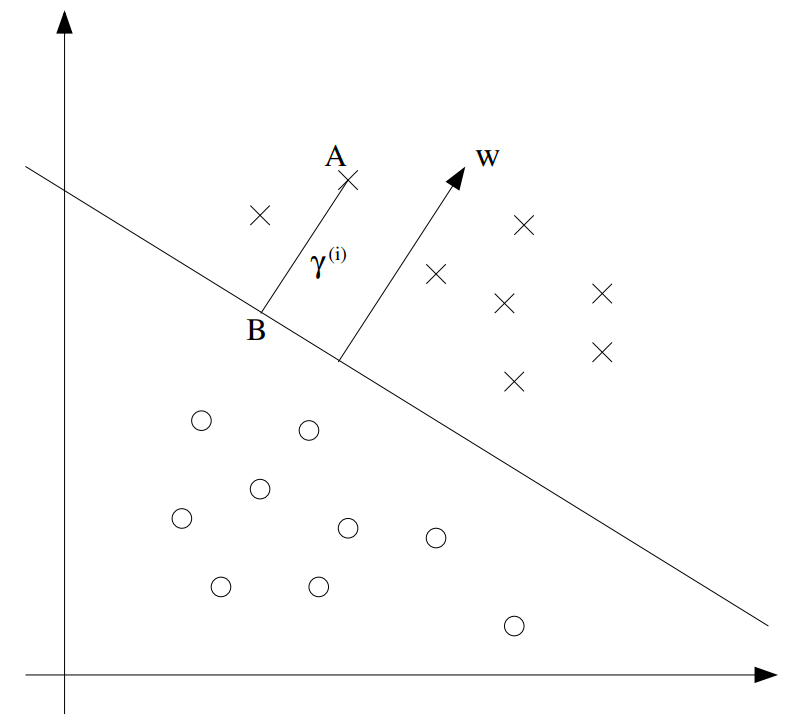
\includegraphics[width=0.5\linewidth]{figs/svm_geo_margin.png}
\end{figure}

图中显示了与 $(w,b)$ 对应的决策边界以及向量 $w$。注意 $w$ 与分隔超平面正交(呈 $90^\circ$ 角)(您应该说服自己确实如此)。 考虑 A 点,它代表标记为 $y^{(i)}=1$ 的某个训练样本的输入 $x^{(i)}$。它到决策边界的距离 $\gamma^{(i)}$ 由线段 AB 给出。

如何找到 $\gamma^{(i)}$ 的值?$w/||w||$ 是一个单位长度向量,方向与 $w$ 相同。由于 A 代表 $x^{(i)}$,因此可以发现点 B 由 $x^{(i)} - \gamma^{(i)} \cdot w/||w||$ 给出。但这个点位于决策边界上,而决策边界上的所有点 $x$ 都满足方程 $w^T x + b = 0$。因此,
\[
    w^T \left( x^{(i)} - \gamma^{(i)} \frac{w}{||w||} \right) + b = 0.
\]
解出 $\gamma^{(i)}$ 得到
\[
    \gamma^{(i)} = \frac{w^T x^{(i)} + b}{||w||} = \left(\frac{w}{||w||}\right)^T x^{(i)} + \frac{b}{||w||}.
\]
这是针对图中 A 点处正训练样本的情况推导的,其中位于决策边界的“正”侧是好的。更一般地,定义 $(w,b)$ 相对于训练样本 $(x^{(i)}, y^{(i)})$ 的几何间隔为
\[
    \gamma^{(i)} = y^{(i)} \left( \left(\frac{w}{||w||}\right)^T x^{(i)} + \frac{b}{||w||} \right).
\]

注意,如果 $||w|| = 1$,那么函数间隔等于几何间隔——这提供了一种关联这两种不同间隔概念的方式。此外,几何间隔对于参数的缩放是不变的;也就是说,如果用 $2w$ 和 $2b$ 替换 $w$ 和 $b$,那么几何间隔不会改变。这在后面会很有用。具体来说,由于参数缩放的这种不变性,在试图拟合 $w$ 和 $b$ 到训练数据时,可以在不改变任何重要内容的情况下对 $w$ 施加任意缩放约束;例如,可以要求 $||w|| = 1$,或者 $|w_1| = 5$,或者 $|w_1 + b| + |w_2| = 2$,并且这些都可以通过缩放 $w$ 和 $b$ 简单地满足。

最后,给定一个训练集 $S = \{(x^{(i)}, y^{(i)}); i = 1, \dots, n\}$,还定义 $(w,b)$ 相对于 $S$ 的几何间隔为各个训练样本的几何间隔中的最小值:
\[
    \gamma = \min_{i=1,\dots,n} \gamma^{(i)}.
\]

\section{最优间隔分类器 (选读)}

给定一个训练集,从之前的讨论来看,一个自然期望是找到一个决策边界,使其几何间隔最大化,因为这将反映一组在训练集上非常确信的预测,并且其能很好地“拟合”训练数据。具体来说,这将产生一个分类器,它用一个“间隔”(几何间隔)来分隔正训练样本和负训练样本。

目前,假设给定一个线性可分的训练集;也就是说,可以通过某个分隔超平面来分隔正样本和负样本。如何找到能实现最大几何间隔的那个呢?可以提出以下优化问题:
\begin{align*}
    \max_{\gamma, w, b} \quad &\gamma\\
    \text{s.t.} & y^{(i)}(w^T x^{(i)} + b) \ge \gamma, \quad i = 1, \dots, n\\
    &||w|| = 1.
\end{align*}
也就是说,希望最大化 $\gamma$,约束条件是每个训练样本的函数间隔至少为 $\gamma$。此外,$||w|| = 1$ 约束确保了函数间隔等于几何间隔,因此也保证了所有几何间隔至少为 $\gamma$。因此,解决这个问题将得到 $(w,b)$,使其相对于训练集具有最大的可能几何间隔。

如果能解决上面的优化问题,任务就完成了。但是,“$||w|| = 1$” 是一个令人讨厌的(非凸)约束,并且这种问题肯定不是标准优化软件可以解决的格式。因此,尝试将问题转换为更友好的形式。考虑:
\begin{align*}
    \max_{\gamma, w, b} \quad &\frac{\hat\gamma}{||w||}\\
    \text{s.t.} \quad & y^{(i)}(w^T x^{(i)} + b) \ge \hat\gamma, \quad i = 1, \dots, n
\end{align*}
这里,要最大化 $\hat{\gamma}/||w||$,约束条件是所有函数间隔至少为 $\hat{\gamma}$。由于几何间隔和函数间隔通过 $\gamma = \hat{\gamma}/||w||$ 相关,这将得到想要的答案。此外,摆脱了不喜欢的 $||w|| = 1$ 约束。缺点是现在有一个令人讨厌的(还是非凸的)目标函数 $\frac{\hat{\gamma}}{||w||}$;而且,仍然没有现成的软件可以解决这种形式的优化问题。

再想想。回想之前关于可以在不改变任何内容的情况下对 $w$ 和 $b$ 添加任意缩放约束的讨论。这是现在要使用的关键思想。引入缩放约束,使得 $(w,b)$ 相对于训练集的函数间隔必须为 1:
\[
    \hat{\gamma} = 1.
\]
由于将 $w$ 和 $b$ 乘以某个常数会导致函数间隔也乘以相同的常数,这确实是一个缩放约束,并且可以通过缩放 $w, b$ 来满足。将其代入上面的问题,并注意到最大化 $\hat{\gamma}/||w|| = 1/||w||$ 等价于最小化 $||w||^2$,现在有了以下优化问题:
\begin{align*}
    \min_{w, b} \quad &\frac{1}{2}||w||^2\\
    \text{s.t.} \quad & y^{(i)}(w^T x^{(i)} + b) \ge \hat\gamma, \quad i = 1, \dots, n
\end{align*}

现在已经将问题转换成可以有效求解的形式。上述问题是一个具有凸二次目标函数和线性约束的优化问题。其解给出了\textbf{最优间隔分类器 (optimal margin classifier)}。可以使用商用二次规划(QP)代码来解决此优化问题\footnote{您可能熟悉线性规划,它解决具有目标函数和约束均是线性的优化问题。QP 软件也广泛可用,它允许具有凸二次目标函数和线性约束。}。

虽然可以称此问题已解决,但下文会进一步讨论拉格朗日对偶性。这将导出优化问题的对偶形式,使得我们可以应用核函数让最优间隔分类器在极高维空间中高效工作。对偶形式还将允许推导出一种求解上述优化问题的高效算法,该算法通常比通用 QP 软件表现更好。

\section{拉格朗日对偶性 (选读)}

暂时搁置支持向量机和最大间隔分类器,讨论如何解决带约束的优化问题。

考虑以下形式的问题:
\begin{align*}
    \min_w \quad &f(w)\\
    \text{s.t.} \quad &h_i(w)=0,\quad i=1,\dots,l.
\end{align*}
一些读者可能还记得如何使用拉格朗日乘数法来解决此问题。(如果以前没有见过,不用担心。)在此方法中,定义\textbf{拉格朗日函数 (Lagrangian)} 为
\[
    \mathcal{L}(w, \beta) = f(w) + \sum_{i=1}^l \beta_i h_i(w)
\]
这里,$\beta_i$ 称为\textbf{拉格朗日乘数 (Lagrange multipliers)}。然后找到 $\mathcal{L}$ 的偏导数并将其设为零:
\[
    \frac{\partial \mathcal{L}}{\partial w_i} = 0; \quad \frac{\partial \mathcal{L}}{\partial \beta_i} = 0,
\]
并求解 $w$ 和 $\beta$。

在本节中,将此推广到可能包含不等式约束和等式约束的优化问题。由于时间限制,无法在本课程中充分论述拉格朗日对偶性理论\footnote{对学习更多关于此主题感兴趣的读者,建议阅读,例如,R. T. Rockafeller (1970), Convex Analysis, Princeton University Press.},但将给出主要思想和结果,并将其应用于最优间隔分类器的优化问题。

考虑以下问题,将其称为\textbf{原始 (primal)} 优化问题:

\begin{align*}
    \min_w \quad &f(w)\\
    \text{s.t.} \quad &g_i(w)\leq 0, \quad i=1,\dots,k\\
    \quad &h_i(w)=0, \quad i=1,\dots,l.
\end{align*}
为了解决它,首先定义\textbf{广义拉格朗日函数 (generalized Lagrangian)}:
\[
    \mathcal{L}(w, \alpha, \beta) = f(w) + \sum_{i=1}^k \alpha_i g_i(w) + \sum_{i=1}^l \beta_i h_i(w).
\]
这里,$\alpha_i$ 和 $\beta_i$ 是拉格朗日乘数。考虑以下量
\[
    \theta_{\mathcal{P}}(w) = \max_{\alpha, \beta: \alpha_i \ge 0} \mathcal{L}(w, \alpha, \beta).
\]
这里,下标 “$\mathcal{P}$” 代表 “原始”。给定某个 $w$。如果 $w$ 违反任何原始约束(即,对于某个 $i$,要么 $g_i(w) > 0$ 要么 $h_i(w) \ne 0$),那么应该能够验证
\begin{align}
    \theta_{\mathcal{P}}(w) &= \max_{\alpha, \beta: \alpha_i \ge 0} f(w) + \sum_{i=1}^k \alpha_i g_i(w) + \sum_{i=1}^l \beta_i h_i(w) \label{eq:6.1} \\
    &= \infty. \label{eq:6.2}
\end{align}
反之,如果约束对于某个特定的 $w$ 值确实满足,那么 $\theta_{\mathcal{P}}(w) = f(w)$。因此,
\[
    \theta_{\mathcal{P}}(w) = \begin{cases} f(w) & \text{若 } w \text{ 满足原始约束} \\ \infty & \text{其他情况}. \end{cases}
\]
因此,对于满足原始约束的所有 $w$ 值,$\theta_{\mathcal{P}}$ 取与问题中目标函数相同的值,如果违反约束,则为正无穷大。因此,如果考虑最小化问题
\[
    \min_w \theta_{\mathcal{P}}(w) = \min_w \max_{\alpha, \beta: \alpha_i \ge 0} \mathcal{L}(w, \alpha, \beta),
\]
可以看出它与原始问题相同(即,具有与原始问题相同的解)。为了后续使用,还将目标函数的最优值定义为 $p^* = \min_w \theta_{\mathcal{P}}(w)$;将其称为原始问题的\textbf{值 (value)}。

现在,考察一个稍微不同的问题。定义
\[
    \theta_{\mathcal{D}}(\alpha, \beta) = \min_w \mathcal{L}(w, \alpha, \beta).
\]
这里,下标 “$\mathcal{D}$” 代表 “对偶”。注意,在 $\theta_{\mathcal{P}}$ 的定义中,关于 $\alpha, \beta$ 进行优化(最大化),而这里关于 $w$ 进行最小化。

现在可以提出\textbf{对偶 (dual)} 优化问题:
\[
    \max_{\alpha, \beta: \alpha_i \ge 0} \theta_{\mathcal{D}}(\alpha, \beta) = \max_{\alpha, \beta: \alpha_i \ge 0} \min_w \mathcal{L}(w, \alpha, \beta).
\]
这与上面显示的原始问题完全相同,只是 “max” 和 “min” 的顺序现在交换了。将对偶问题目标函数的最优值定义为 $d^* = \max_{\alpha, \beta: \alpha_i \ge 0} \theta_{\mathcal{D}}(w)$。

原始问题和对偶问题如何关联?很容易证明
\[
    d^* = \max_{\alpha, \beta: \alpha_i \ge 0} \min_w \mathcal{L}(w, \alpha, \beta) \le \min_w \max_{\alpha, \beta: \alpha_i \ge 0} \mathcal{L}(w, \alpha, \beta) = p^*.
\]
(您应该自己证明这一点;这源自函数 “max min” 总是小于或等于 “min max”。)然而,在某些条件下,将有
\[
    d^* = p^*,
\]
这样就可以求解对偶问题来代替原始问题。来看看这些条件是什么。

假设 $f$ 和 $g_i$ 是凸函数\footnote{当 $f$ 具有 Hessian 矩阵时,当且仅当 Hessian 矩阵是半正定时,它是凸的;类似地,所有线性(和仿射)函数也是凸的。(函数 $f$ 也可以在不可微的情况下是凸的,但这里不需要那些更一般的凸性定义。)},并且 $h_i$ 是仿射函数\footnote{即,存在 $a_i, b_i$,使得 $h_i(w) = a_i^T w + b_i$。“仿射”的意思与线性相同,只是允许额外的截距项 $b_i$。}。进一步假设约束 $g_i$ 是(严格)可行的;这意味着存在某个 $w$ 使得对于所有 $i$,都有 $g_i(w) < 0$。

在上述假设下,必然存在 $w^*, \alpha^*, \beta^*$,使得 $w^*$ 是原始问题的解,$\alpha^*, \beta^*$ 是对偶问题的解,并且 $p^* = d^* = \mathcal{L}(w^*, \alpha^*, \beta^*)$。此外,$w^*, \alpha^*$ 和 $\beta^*$ 满足 \textbf{Karush-Kuhn-Tucker (KKT) 条件},如下:
\begin{align}
    \frac{\partial}{\partial w_i} \mathcal{L}(w^*, \alpha^*, \beta^*) &= 0, \quad i = 1, \dots, d \label{eq:6.3} \\
    \frac{\partial}{\partial \beta_i} \mathcal{L}(w^*, \alpha^*, \beta^*) &= 0, \quad i = 1, \dots, l \label{eq:6.4} \\
    \alpha_i^* g_i(w^*) &= 0, \quad i = 1, \dots, k \label{eq:6.5} \\
    g_i(w^*) &\le 0, \quad i = 1, \dots, k \label{eq:6.6} \\
    \alpha^* &\ge 0, \quad i = 1, \dots, k \label{eq:6.7}
\end{align}
此外,如果某个 $w^*, \alpha^*, \beta^*$ 满足 KKT 条件,那么它也是原始问题和对偶问题的解。

请注意方程 (\ref{eq:6.5}),它被称为 KKT \textbf{对偶互补性条件 (dual complementarity)}。具体来说,这意味着如果 $\alpha_i^* > 0$,那么 $g_i(w^*) = 0$。(即,“$g_i(w) \le 0$” 约束是\textbf{活跃 (active)} 的,意味着它以等式而不是不等式成立。)稍后,这将是证明 SVM 只有少量“支持向量”的关键;KKT 对偶互补性条件也将为讨论 SMO 算法时提供收敛性测试。

\section{最优间隔分类器:对偶形式 (选读)}

\textcolor{blue}{注:}\textit{优化问题 \eqref{eq:primal_opt} 与优化问题 \eqref{eq:dual_opt} 的等价性,以及方程 \eqref{eq:dual_relation} 中原始变量和对偶变量之间的关系是本节最重要的收获。}

前面,提出了以下寻找最优间隔分类器的问题(原始)优化问题:
\begin{align}
    \min_{w,b} \quad &\frac{1}{2}\|w\|^2 \label{eq:primal_opt}\\
    \text{s.t.} \quad &y^{(i)}(w^T x^{(i)} + b) \ge 1, \quad i = 1, \dots, n \notag
\end{align}
可以将约束写成
\[
    g_i(w) = -y^{(i)}(w^T x^{(i)} + b) + 1 \le 0.
\]
每个训练样本都有一个这样的约束。注意,根据 KKT 对偶互补性条件,只有当训练样本的功能间隔恰好等于 1 时(即,对应于满足等式 $g_i(w) = 0$ 的约束),$\alpha_i$ 才大于 0。考虑下图中,其中实线表示最大间隔分离超平面。

\begin{figure}[H]
    \centering
    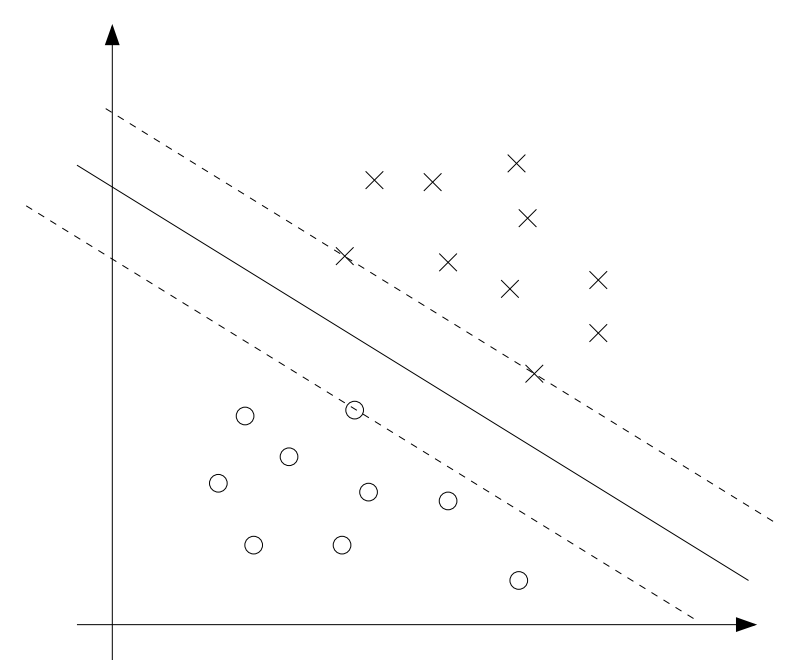
\includegraphics[width=0.5\linewidth]{figs/svm_max_margin.png}
\end{figure}

间隔最小的点恰好是离决策边界最近的点;在这里,这三个点(一个负样本和两个正样本)位于平行于决策边界的虚线上。因此,只有这三个 $\alpha_i$(即,对应于这三个训练样本的 $\alpha_i$)在最优解处非零。这三个点被称为该问题中的\textbf{支持向量 (support vectors)}。支持向量的数量可以远小于训练集的大小,这一事实将在稍后有用。

接下来,在推导对偶形式问题时,需要注意的一个关键思想是,我们将尝试仅使用内积 $\langle x^{(i)}, x^{(j)} \rangle$(将其视为输入特征空间中点之间的 $(x^{(i)})^T x^{(j)}$)来编写算法。算法能够用这些内积表达的事实是应用核技巧的关键。

构建优化问题的拉格朗日函数为:
\begin{equation}
    \mathcal{L}(w, b, \alpha) = \frac{1}{2}\|w\|^2 - \sum_{i=1}^n \alpha_i [y^{(i)}(w^T x^{(i)} + b) - 1]. \label{eq:la_opt}
\end{equation}
注意,只有“$\alpha_i$”而没有“$\beta_i$”拉格朗日乘子,因为问题只有不等式约束。

继续推导问题的对偶形式。为此,需要首先对固定的 $\alpha$ 最小化 $\mathcal{L}(w, b, \alpha)$ 关于 $w$ 和 $b$,以得到 $\theta_D$。方法是将 $\mathcal{L}$ 关于 $w$ 和 $b$ 的导数设为零。得到:
\[
    \nabla_w \mathcal{L}(w, b, \alpha) = w - \sum_{i=1}^n \alpha_i y^{(i)} x^{(i)} = 0
\]
这意味着
\begin{equation}
    w = \sum_{i=1}^n \alpha_i y^{(i)} x^{(i)}. \label{eq:dual_relation}
\end{equation}
关于 $b$ 的导数,得到
\begin{equation}
    \frac{\partial}{\partial b} \mathcal{L}(w, b, \alpha) = \sum_{i=1}^n \alpha_i y^{(i)} = 0. \label{eq:6.11}
\end{equation}
将式 \eqref{eq:dual_relation} 中 $w$ 的定义代入拉格朗日函数 \eqref{eq:la_opt},并简化,得到
\[
    \mathcal{L}(w, b, \alpha) = \sum_{i=1}^n \alpha_i - \frac{1}{2} \sum_{i,j=1}^n y^{(i)} y^{(j)} \alpha_i \alpha_j (x^{(i)})^T x^{(j)} - b \sum_{i=1}^n \alpha_i y^{(i)}.
\]
但根据式 \eqref{eq:6.11},最后一项必须为零,所以得到
\[
    \mathcal{L}(w, b, \alpha) = \sum_{i=1}^n \alpha_i - \frac{1}{2} \sum_{i,j=1}^n y^{(i)} y^{(j)} \alpha_i \alpha_j (x^{(i)})^T x^{(j)}.
\]
回想一下,通过对 $\mathcal{L}$ 关于 $w$ 和 $b$ 进行最小化,得到了上面的方程。将其与约束 $\alpha_i \ge 0$(始终存在)和约束 \eqref{eq:6.11} 结合,得到以下对偶优化问题:
\begin{align}
    \max_\alpha \quad &W(\alpha) = \sum_{i=1}^n \alpha_i - \frac{1}{2} \sum_{i,j=1}^n y^{(i)} y^{(j)} \alpha_i \alpha_j \langle x^{(i)}, x^{(j)} \rangle \label{eq:dual_opt} \\
    \text{s.t.} \quad & \alpha_i \ge 0, \quad i=1,\dots,n \notag\\
     & \sum_{i=1}^n \alpha_i y^{(i)} = 0. \notag
\end{align}

还应该能够验证 $p^* = d^*$ 所需的条件以及 KKT 条件(式 \eqref{eq:6.3}-\eqref{eq:6.7})在我们的优化问题里确实满足。因此,可以通过求解对偶问题来求解原问题。具体而言,在上述对偶问题中,这是一个最大化问题,其中的参数是 $\alpha_i$。稍后将讨论用于求解对偶问题的具体算法,但如果确实能够求解它(即找到使 $W(\alpha)$ 最大化且满足约束的 $\alpha$),那么就可以使用式 \eqref{eq:dual_relation} 回过头来找到最优的 $w$ 作为 $\alpha$ 的函数。找到 $w^*$ 后,通过考虑原问题,也很容易找到截距项 $b$ 的最优值,如下所示:
\begin{equation}
    b^* = - \frac{\max_{i:y^{(i)}=-1} w^{*T} x^{(i)} + \min_{i:y^{(i)}=1} w^{*T} x^{(i)}}{2}. \label{eq:6.13}
\end{equation}
(可以自行验证一下此处的正确性。)

继续之前,再仔细看看式 \eqref{eq:dual_relation},它给出了 $w$ 的最优值(以最优 $\alpha$ 表示)。假设已经用训练集拟合了模型参数,现在想对新的输入点 $x$ 进行预测。然后计算 $w^T x + b$,并且当且仅当该值大于零时预测 $y=1$。但是使用 \eqref{eq:dual_relation},该值也可以写成:
\begin{align}
    w^T x + b &= \left(\sum_{i=1}^n \alpha_i y^{(i)} x^{(i)}\right)^T x + b \\
    &= \sum_{i=1}^n \alpha_i y^{(i)} \langle x^{(i)}, x \rangle + b. \label{eq:6.15}
\end{align}
因此,如果找到了 $\alpha_i$,为了进行预测,必须计算一个仅取决于 $x$ 与训练集中的点之间的内积的值。此外,之前已经看到,除了支持向量对应的 $\alpha_i$ 外,其他所有 $\alpha_i$ 都将为零。因此,上面求和中的许多项将为零,并且实际上只需要计算 $x$ 与支持向量(通常数量很少)之间的内积,以便计算 \eqref{eq:6.15} 并进行预测。

通过研究优化问题的对偶形式,对问题的结构获得了重要的见解,并且还能够仅以内积形式编写整个算法。在下一节中,将利用这一特性将核函数应用于分类问题。由此产生的算法,\textbf{支持向量机 (support vector machines)},将能够在非常高维的空间中高效学习。

\section{正则化与非线性可分情况 (选读)}

目前为止介绍的支持向量机推导假设数据是线性可分的。虽然通过 $\phi$ 将数据映射到高维特征空间通常会增加数据可分的可能性,但不能保证总是如此。此外,在某些情况下,找到一个分离超平面并非完全符合期望,因为它可能对离群点敏感。例如,下面左图显示了一个最优间隔分类器,当在左上方区域(右图)添加一个离群点时,决策边界会发生剧烈变化,并且得到的分类器的间隔会小得多。

\begin{figure}[H]
    \centering
    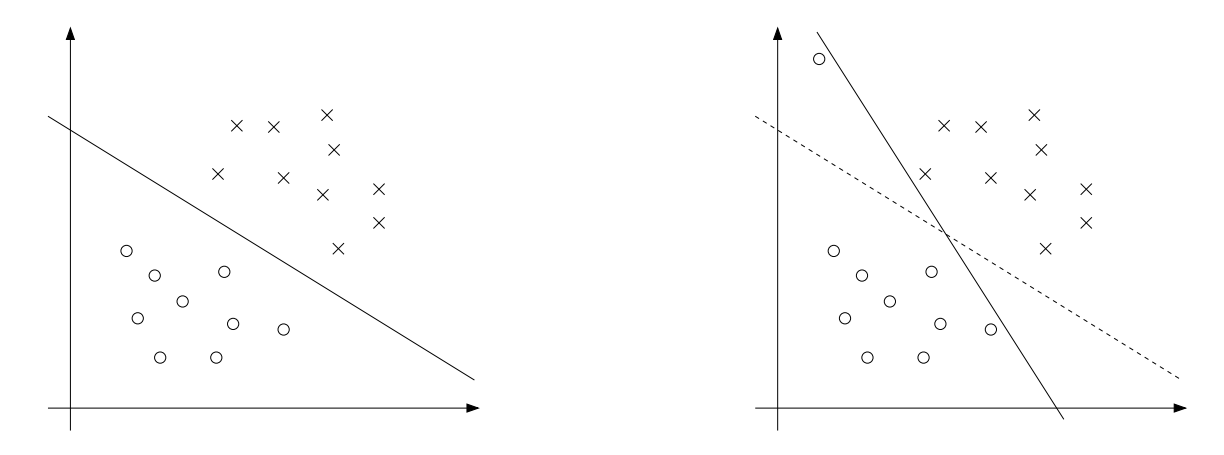
\includegraphics[width=0.93\linewidth]{figs/svm_regularization.png}
\end{figure}

为了使算法也适用于非线性可分数据集并降低对离群点的敏感度,我们重新构建了优化问题(使用 $\ell_1$ \textbf{正则化 (regularization)}),如下所示:
\begin{align*}
    \min_{\gamma,w,b} \quad& \frac{1}{2}\|w\|^2 + C \sum_{i=1}^n \xi_i \\
    \text{s.t.} \quad& y^{(i)}(w^T x^{(i)} + b) \ge 1 - \xi_i, \quad i=1,\dots,n \\
    &\xi_i \ge 0, \quad i=1,\dots,n.
\end{align*}
因此,现在允许存在(函数)间隔小于 1 的样本,如果一个样本的函数间隔为 $1-\xi_i$(其中 $\xi_i > 0$),那么目标函数会增加 $C\xi_i$ 的代价。参数 $C$ 控制了两个目标之间的相对权重:使 $\|w\|^2$ 小(如前面所述,这会使间隔大)以及确保大多数样本的函数间隔至少为 1。

与之前一样,可以构建拉格朗日函数:
\[
    \mathcal{L}(w, b, \xi, \alpha, r) = \frac{1}{2} w^T w + C \sum_{i=1}^n \xi_i - \sum_{i=1}^n \alpha_i [y^{(i)}(w^T x^{(i)} + b) - 1 + \xi_i] - \sum_{i=1}^n r_i \xi_i.
\]
这里,$\alpha_i$ 和 $r_i$ 是拉格朗日乘子(约束为 $\ge 0$)。将不再详细推导对偶问题,但在像之前一样将关于 $w$ 和 $b$ 的导数设为零,然后代入并简化后,得到问题的对偶形式:
\begin{align*}
    \max{\alpha} \quad& W(a)=\sum_{i=1}^{n}a_i - \frac12 \sum_{i,j=1}^n y^{(i)}y^{(j)}\alpha_i\alpha_j\langle x^{(i)}x^{(j)} \rangle \\
    \text{s.t.} \quad& 0\le \alpha_i\le C, \quad i=1,\dots,n \\
    &\sum_{i=1}^{n}\alpha_i y^{(i)}=0.
\end{align*}

与之前一样,同样有 $w$ 可以表示为 $\alpha_i$ 的函数,如式 \eqref{eq:dual_relation} 所示,因此在求解对偶问题后,可以继续使用式 \eqref{eq:6.15} 进行预测。注意,令人惊讶的是,在添加 $\ell_1$ 正则化后,对偶问题唯一的改变是原先的约束 $0 \le \alpha_i$ 现在变成了 $0 \le \alpha_i \le C$。对 $b^*$ 的计算也必须进行修改(式 \eqref{eq:6.13} 不再有效);请参阅下一节中的注释或 Platt 的论文。

此外,KKT 对偶互补条件(在下一节中将用于测试 SMO 算法的收敛性)为:
\begin{align}
    \alpha_i = 0 &\Rightarrow y^{(i)}(w^T x^{(i)} + b) \ge 1 \label{eq:6.16} \\
    \alpha_i = C &\Rightarrow y^{(i)}(w^T x^{(i)} + b) \le 1 \label{eq:6.17} \\
    0 < \alpha_i < C &\Rightarrow y^{(i)}(w^T x^{(i)} + b) = 1. \label{eq:6.18}
\end{align}
现在,剩下的就是给出一个实际求解对偶问题的算法,这将在下一节中进行。

\section{SMO 算法 (选读)}

序列最小化 (sequential minimal optimization, SMO) 算法,由 John Platt 提出,提供了一种有效求解由 SVM 推导得到的对偶问题的方法。部分是为了引出 SMO 算法,部分是因为它本身很有趣,让我们先再进行一次岔开讨论,谈谈坐标上升算法。

\subsection{坐标上升}

考虑尝试求解无约束优化问题
\[
    \max_\alpha W(\alpha_1, \alpha_2, \dots, \alpha_n).
\]
这里,将 $W$ 视为参数 $\alpha_i$ 的某个函数,暂时忽略这个问题与支持向量机之间的任何关系。之前已经见过两种优化算法:梯度上升和牛顿法。这里要考虑的新算法称为\textbf{坐标上升 (coordinate ascent)}:

循环直到收敛: \{

    $\quad\quad$对于 $i=1,\dots,n,$ \{
        \[
            \alpha_i := \arg\max_{\hat a_i} W(\alpha_1,\dots,\alpha_{i-1},\hat{\alpha_i},\alpha_{i+1},\dots,\alpha_n).
        \]
        
    $\quad\quad$\}

\}

因此,在该算法的最内层循环中,将固定除某个 $\alpha_i$ 之外的所有变量,并仅针对参数 $\alpha_i$ 重新优化 $W$。在该方法此处介绍的版本中,内层循环按 $\alpha_1, \alpha_2, \dots, \alpha_n, \alpha_1, \alpha_2, \dots$ 的顺序重新优化变量。(更复杂的版本可以选择其他顺序;例如,可以根据期望哪个变量能使 $W(\alpha)$ 增加最大来选择下一个要更新的变量。)

当函数 $W$ 的形式恰好使得内层循环中的 “arg max” 可以高效执行时,坐标上升可以是一个相当高效的算法。这里是坐标上升算法的一个图例:

\begin{figure}[H]
    \centering
    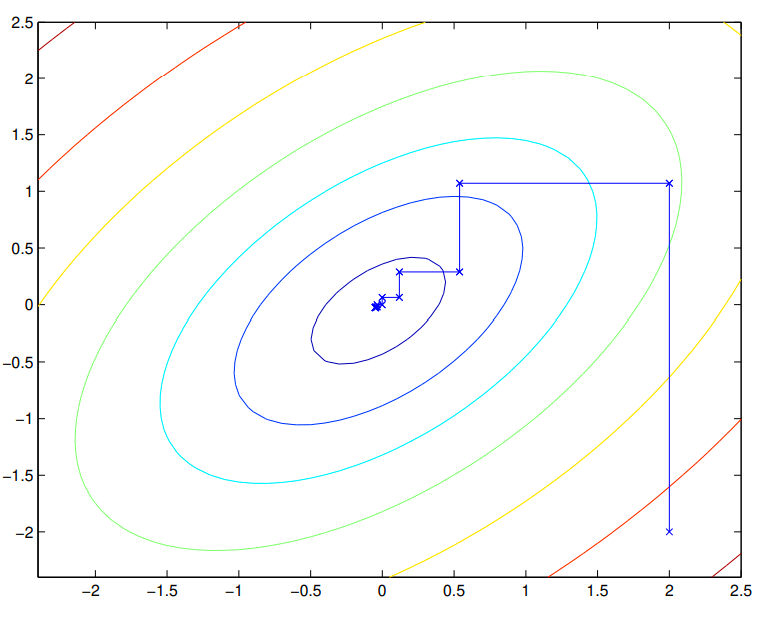
\includegraphics[width=0.5\linewidth]{figs/svm_coordinate_ascent.png}
\end{figure}


图中的椭圆是我们想要优化的二次函数的等高线。坐标上升从 $(2, -2)$ 初始化,图中绘制了它通往全局最大值的路径。注意到在每一步,坐标上升都沿着与一个坐标轴平行的方向前进,因为每次只优化一个变量。

\subsection{SMO}

通过概述 SMO 算法的推导来结束对支持向量机的讨论。

这是我们想要解决的(对偶)优化问题:
\begin{align}
    \max_\alpha \quad &W(\alpha) = \sum_{i=1}^n \alpha_i - \frac{1}{2} \sum_{i,j=1}^n y^{(i)} y^{(j)} \alpha_i \alpha_j \langle x^{(i)}, x^{(j)} \rangle \\
    \text{s.t.} \quad &0 \le \alpha_i \le C, \quad i=1,\dots,n \label{eq:6.20}\\
    &\sum_{i=1}^n \alpha_i y^{(i)} = 0. \label{eq:6.21}
\end{align}

假设我们有一组满足约束 (\eqref{eq:6.20}-\eqref{eq:6.21}) 的 $\alpha_i$。现在,假设我们固定 $\alpha_2, \dots, \alpha_n$,并进行坐标上升步骤,关于 $\alpha_1$重新优化目标函数。能取得任何进展吗?答案是否定的,因为约束 \eqref{eq:6.21} 确保
\[
    \alpha_1 y^{(1)} = - \sum_{i=2}^n \alpha_i y^{(i)}.
\]

或者,通过将两边乘以 $y^{(1)}$,我们等价地得到
\[
    \alpha_1 = -y^{(1)} \sum_{i=2}^n \alpha_i y^{(i)}.
\]
(这一步使用了 $y^{(1)} \in \{-1, 1\}$ 的事实,因此 $(y^{(1)})^2 = 1$。)因此,$\alpha_1$ 完全由其他 $\alpha_i$ 确定,如果固定 $\alpha_2, \dots, \alpha_n$,那么在不违反优化问题中的约束 \eqref{eq:6.21} 的情况下,无法对 $\alpha_1$ 进行任何改变。

因此,如果想要更新一些 $\alpha_i$,必须同时更新至少两个,以便保持约束得到满足。这促使了 SMO 算法,其简单来说就是以下步骤:

\begin{samepage}
重复直到收敛 \{
\vspace{-0.5em}
\begin{enumerate}
\setlength{\itemindent}{2em}
    \item 选择一对 $\alpha_i$ 和 $\alpha_j$ 进行下一次更新(使用启发式方法来选择能够最大程度接近全局最大值的两个变量)。
    \item 在保持所有其他 $\alpha_k$ ($k \ne i, j$) 固定的情况下,重新优化 $W(\alpha)$ 关于 $\alpha_i$ 和 $\alpha_j$。
\end{enumerate}
$\quad\quad$\}
\end{samepage}

为了测试该算法的收敛性,可以检查 KKT 条件(式 \eqref{eq:6.16}-\eqref{eq:6.18})是否在某个 $\textit{容差 (tol)}$ 内得到满足。这里,容差是收敛容差参数,通常设置为 0.01 到 0.001。(详细信息请参阅论文和伪代码。)

SMO 算法高效的关键原因在于 $\alpha_i, \alpha_j$ 的更新可以非常高效地计算。现在简要概述推导高效更新的主要思路。

假设当前有一组满足约束 (\eqref{eq:6.20}-\eqref{eq:6.21}) 的 $\alpha_i$,并且假设决定固定 $\alpha_3, \dots, \alpha_n$,并重新优化 $W(\alpha_1, \alpha_2, \dots, \alpha_n)$ 关于 $\alpha_1$ 和 $\alpha_2$(受约束限制)。根据 \eqref{eq:6.21},我们要求
\[
    \alpha_1 y^{(1)} + \alpha_2 y^{(2)} = - \sum_{i=3}^n \alpha_i y^{(i)}.
\]
由于右侧是固定的(因为已经固定了 $\alpha_3, \dots, \alpha_n$),可以将其记为某个常数 $\zeta$:
\begin{equation}
    \alpha_1 y^{(1)} + \alpha_2 y^{(2)} = \zeta. \label{eq:6.22}
\end{equation}
因此,可以将 $\alpha_1$ 和 $\alpha_2$ 的约束可视化如下:

\begin{figure}[H]
    \centering
    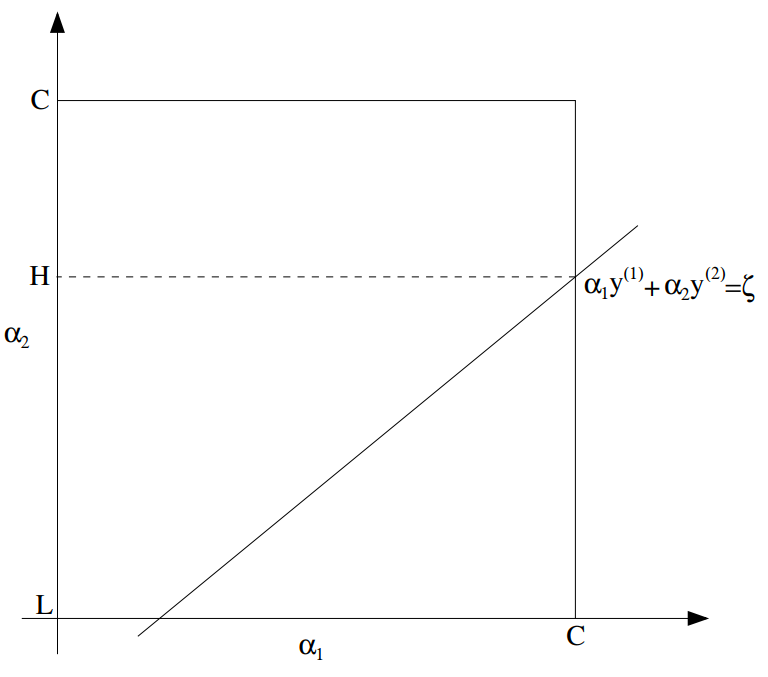
\includegraphics[width=0.5\linewidth]{figs/svm_smo_constraint.png}
\end{figure}

从约束 \eqref{eq:6.20} 中,我们知道 $\alpha_1$ 和 $\alpha_2$ 必须位于所示的盒子 $[0, C] \times [0, C]$ 内。还绘制了直线 $\alpha_1 y^{(1)} + \alpha_2 y^{(2)} = \zeta$,我们知道 $\alpha_1$ 和 $\alpha_2$ 必须位于该直线上。另外注意,从这些约束中,我们知道 $L \le \alpha_2 \le H$;否则,$(\alpha_1, \alpha_2)$ 无法同时满足盒子约束和直线约束。在此示例中,$L=0$。但这取决于直线 $\alpha_1 y^{(1)} + \alpha_2 y^{(2)} = \zeta$ 的样子,情况并非总是如此;更普遍地,对于 $\alpha_2$ 的允许值,会有一个下界 $L$ 和一个上界 $H$,以确保 $\alpha_1, \alpha_2$ 位于盒子 $[0, C] \times [0, C]$ 内。

使用方程 \eqref{eq:6.22},我们还可以将 $\alpha_1$ 写成 $\alpha_2$ 的函数:
\[
    \alpha_1 = (\zeta - \alpha_2 y^{(2)}) y^{(1)}.
\]
(请自行验证此推导;我们再次使用了 $y^{(1)} \in \{-1, 1\}$ 的事实,因此 $(y^{(1)})^2 = 1$。)因此,目标函数 $W(\alpha)$ 可以写成
\[
    W(\alpha_1, \alpha_2, \dots, \alpha_n) = W((\zeta - \alpha_2 y^{(2)}) y^{(1)}, \alpha_2, \dots, \alpha_n).
\]
将 $\alpha_3, \dots, \alpha_n$ 视为常数,您应该能够验证这是关于 $\alpha_2$ 的二次函数。也就是说,这也可以表示为 $a\alpha_2^2 + b\alpha_2 + c$ 的形式,其中 $a, b, c$ 是适当的常数。如果忽略“盒子”约束 \eqref{eq:6.20}(或等价地,忽略 $L \le \alpha_2 \le H$),那么我们可以通过将其导数设为零并求解来轻松最大化此二次函数。我们将令 $\alpha_2^{\text{new,unclipped}}$ 表示由此产生的 $\alpha_2$ 值。您还应该能够说服自己,如果改为最大化关于 $\alpha_2$ 的 $W$,但受盒子约束限制,那么可以通过简单地取 $\alpha_2^{\text{new,unclipped}}$ 并将其“剪裁”到$[L, H]$ 区间内,得到
\[
    \alpha_2^{\text{new}} = \begin{cases}
        H & \text{若}\  \alpha_2^{\text{new,unclipped}} > H \\
        \alpha_2^{\text{new,unclipped}} & \text{若}\  L \le \alpha_2^{\text{new,unclipped}} \le H \\
        L & \text{若}\  \alpha_2^{\text{new,unclipped}} < L
    \end{cases}
\]
最后,找到 $\alpha_2^{\text{new}}$ 后,可以使用方程 \eqref{eq:6.22} 返回并找到 $\alpha_1^{\text{new}}$ 的最优值。

还有一些细节非常简单,但我们将留给您自己在 Platt 的论文中阅读:一个是用于选择下一个要更新的 $\alpha_i, \alpha_j$ 的启发式方法的选择;另一个是 SMO 算法运行时如何更新 $b$。